\chapter{Datos de Panel}

El dato verdadero de panel se trata de tener una serie continua a lo largo del tiempo, esto a diferencia de los datos pooled cross-section, que se trata de poner un dato debajo de otro.

$$y_{it} = \beta_0+\beta_1x_{it1}+\cdots + \beta_k x_{itk} + u_{it}$$

Donde:

\begin{itemize}
	\item $t= 1,2,\cdots, T$ es el tiempo.
	\item $i= 1,2,\cdots, N$ es el número de unidades.
\end{itemize}

Existen dos clases de paneles:

\begin{itemize}
    \item Paneles micro. Siempre que $t<N$. (30000 empresas y 10 años).
    \item Paneles macro. Siempre que $t\approx N$. (30 países y 30 años).
\end{itemize}

Un panel es \textbf{balanceado} si todas las unidades tienen la misma cantidad de observaciones. Y es \textbf{desbalanceado} si no todas las unidades tienen la misma cantidad de observaciones.

Con respecto a pooled cross-section,
\begin{itemize}
    \item Lo utilizamos para investigar el efecto del tiempo.
    \item Lo utilizaremos si hay relaciones en el tiempo.
\end{itemize}

\section{Chapter 13: Pooling Cross-Sections Across Time, Simple Panel Data Methods}

En este ejemplo responderemos a:
\begin{center}
    ¿Ha variado la fertilidad de las mujeres en el tiempo?
\end{center}

Utilizaremos datos de 1129 mujeres, que le preguntaremos cuantos hijos tiene. Tendremos datos para 7 años cada 2 años. Colocaremos las variables ficticias para no entrar en la trampa de variables ficticias.

\subsection{Variables ficticias}
Nunca podemos poner todas las categorías al mismo tiempo, ya que tendríamos multicolinialidad exacta. Por lo que al aplicar MCO no podríamos estimar los coeficientes.

\begin{center}
Modelo 1: MCO, usando las observaciones 1--1129\\
Variable dependiente: kids\\

\vspace{1em}

\begin{tabular}{lr@{,}lr@{,}lr@{,}lr@{,}l}
  &
 \multicolumn{2}{c}{Coeficiente} &
  \multicolumn{2}{c}{Desv.\ Típica} &
   \multicolumn{2}{c}{Estadístico $t$} &
    \multicolumn{2}{c}{valor p} \\[1ex]
const &
  $-$7&74246 &
    3&05177 &
      $-$2&537 &
        0&0113 \\
educ &
  $-$0&128427 &
    0&0183486 &
      $-$6&999 &
        0&0000 \\
age &
  0&532135 &
    0&138386 &
      3&845 &
        0&0001 \\
agesq &
  $-$0&00580400 &
    0&00156428 &
      $-$3&710 &
        0&0002 \\
black &
  1&07566 &
    0&173536 &
      6&198 &
        0&0000 \\
east &
  0&217324 &
    0&132788 &
      1&637 &
        0&1020 \\
northcen &
  0&363114 &
    0&120897 &
      3&004 &
        0&0027 \\
west &
  0&197603 &
    0&166913 &
      1&184 &
        0&2367 \\
farm &
  $-$0&0525575 &
    0&147190 &
      $-$0&3571 &
        0&7211 \\
othrural &
  $-$0&162854 &
    0&175442 &
      $-$0&9282 &
        0&3535 \\
town &
  0&0843532 &
    0&124531 &
      0&6774 &
        0&4983 \\
smcity &
  0&211879 &
    0&160296 &
      1&322 &
        0&1865 \\
y74 &
  0&268183 &
    0&172716 &
      1&553 &
        0&1208 \\
y76 &
  $-$0&0973795 &
    0&179046 &
      $-$0&5439 &
        0&5866 \\
y78 &
  $-$0&0686665 &
    0&181684 &
      $-$0&3779 &
        0&7055 \\
y80 &
  $-$0&0713053 &
    0&182771 &
      $-$0&3901 &
        0&6965 \\
y82 &
  $-$0&522484 &
    0&172436 &
      $-$3&030 &
        0&0025 \\
y84 &
  $-$0&545166 &
    0&174516 &
      $-$3&124 &
        0&0018 \\
\end{tabular}

\vspace{1ex}
\begin{tabular}{lrlr}
Media de la vble. dep. &  2,743136 & D.T. de la vble. dep. &  1,653899 \\
Suma de cuad. residuos &  2685,898 & D.T. de la regresión &  1,554847 \\
$R^2$ &  0,129512 & $R^2$ corregido &  0,116192 \\
$F(17, 1111)$ &  9,723282 & Valor p (de $F$) &  2,42\textrm{e--24} \\
Log-verosimilitud & $-$2091,224 & Criterio de Akaike &  4218,448 \\
Criterio de Schwarz &  4308,972 & Hannan--Quinn &  4252,650 \\
\end{tabular}
\end{center}

% importar imagen
\begin{center}
    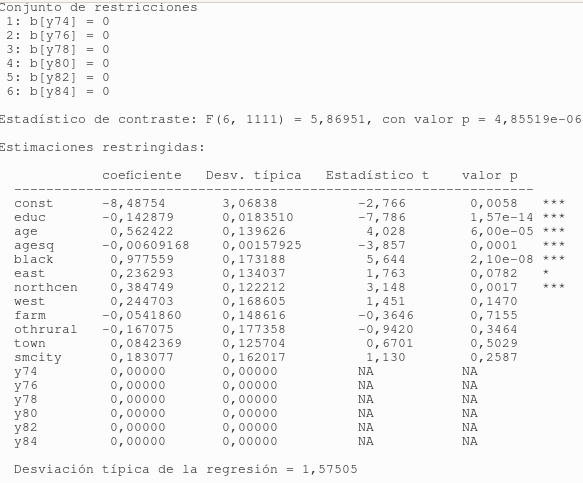
\includegraphics[scale = .5]{./image/kids_contraste_gretl.png}
\end{center}

Se rechaza la hipótesis nula de que los coeficientes de las variables ficticias son iguales a 0. Por lo que se rechaza la hipótesis nula de que la fertilidad de las mujeres no ha variado en el tiempo.


\section{Ejemplo 13.2}

\begin{center}
    ¿Podemos encontrar diferencias salariales por género según la educación?
\end{center}

Serán datos para 78 y 85. Trataremos de predecir los salarios.

\subsection{Efectos de interacción}


\begin{center}

Modelo 1: MCO, usando las observaciones 1--1084\\
Variable dependiente: lwage\\

\vspace{1em}

\begin{tabular}{lr@{,}lr@{,}lr@{,}lr@{,}l}
  &
 \multicolumn{2}{c}{Coeficiente} &
  \multicolumn{2}{c}{Desv.\ Típica} &
   \multicolumn{2}{c}{Estadístico $t$} &
    \multicolumn{2}{c}{valor p} \\[1ex]
const &
  0&458933 &
    0&0934485 &
      4&911 &
        0&0000 \\
y85 &
  0&117806 &
    0&123782 &
      0&9517 &
        0&3415 \\
educ &
  0&0747209 &
    0&00667643 &
      11&19 &
        0&0000 \\
y85edu &
  0&0184605 &
    0&00935417 &
      1&974 &
        0&0487 \\
exper &
  0&0295843 &
    0&00356731 &
      8&293 &
        0&0000 \\
expersq &
  $-$0&000399428 &
    7&75391\textrm{e--05} &
      $-$5&151 &
        0&0000 \\
union &
  0&202132 &
    0&0302945 &
      6&672 &
        0&0000 \\
female &
  $-$0&316709 &
    0&0366214 &
      $-$8&648 &
        0&0000 \\
y85fem &
  0&0850520 &
    0&0513090 &
      1&658 &
        0&0977 \\
\end{tabular}

\vspace{1ex}
\begin{tabular}{lrlr}
Media de la vble. dep. &  1,867301 & D.T. de la vble. dep. &  0,542804 \\
Suma de cuad. residuos &  183,0991 & D.T. de la regresión &  0,412704 \\
$R^2$ &  0,426186 & $R^2$ corregido &  0,421915 \\
$F(8, 1075)$ &  99,80353 & Valor p (de $F$) &  4,5\textrm{e--124} \\
Log-verosimilitud & $-$574,2443 & Criterio de Akaike &  1166,489 \\
Criterio de Schwarz &  1211,384 & Hannan--Quinn &  1183,485 \\
\end{tabular}
\end{center}

Dado que female es negativo, existe un efecto negativo en los salarios. 

En el año base 78, ser mujer disminuye el salario en 0.3. En el año 85, ser mujer es -0.3+0.08 = -0.22. Por lo que el efecto de ser mujer aumenta en 0.08.

La educación tiene un efecto positivo en el salario en el año 78. Ahora ¿Es más importante estudiar en el año 85 o en el 78?: Es mas importante estudiar en el año 85, ya que el efecto de la educación se refuerza en 0.018.

\section{Diferencias en diferencias}

\begin{itemize}
    \item Un experimento natural es por ejemplo los experimentos médicos, donde el existe un grupo de control y un grupo de tratamiento.
    \item En economía, un experimento natural es por ejemplo el efecto de un cambio en la política económica, donde se compara un grupo de control y un grupo de tratamiento.
\end{itemize}
